
\section{Data illustrations\label{sec:results}}

\subsection{Simulations\label{subsec:simulated}}
We have introduced this projected gamma distribution existing on $\mathcal{S}_{\infty}^{p-1}$.  As a
  means of evaluating how well we can recover a distribution under the proposed model, we have
  generated a series of datasets on $\mathcal{S}_{\infty}^{d-1}$, for $d$ ranging between 3 and 20.
  We generated each dataset from a mixture of projected Gammas, with the number of mixture components
  ranging between 3 and 12.  The generation procedure is detailed in Algorithm~\ref{algo:simulated}.
  \begin{algorithm}[ht]
    \caption{Simulated Angular Dataset Generation Routine\label{algo:simulated}}
    \For{$n_{\text{mix}}$ in $[3, 6, 9, 12]$}{
      Generate $n_{\text{mix}} \times 20$ shape Parameters $\alpha$\\
      Generate $n_{\text{mix}} \times 20$ Rate Parameters $\beta$\\
      Generate $500$ Mixture Component Identifiers $\delta$\\
      \For{$i$ in $1,\ldots,500$}{
        Generate ${\bf X}_i \sim \prod_{\ell = 1}^d\text{Ga}\left(X_{il}\mid\alpha_{\delta_i,l},\beta_{\delta_i, l}\right)$
        }
      \For{$n_{\text{col}}$ in $[3,6,12,20]$}{
        Project columns 1 to $n_{\text{col}}$ of ${\bf X}$ onto 
        $\mathcal{S}_{\infty}^{n_{\text{col}} - 1}$ and save.
        }
    }
  \end{algorithm}
  The choice of generation routine for $\alpha = \alpha_0 + \alpha_1$ where
  $\alpha_0 \sim \text{Unif}(\alpha_0\mid 0,4)$, $\alpha_1\sim \text{Gamma}(\alpha_1\mid 1,1)$.
  The choice of generation routine for $\beta$ is $\beta\sim\text{Unif}(\beta\mid 0.25, 2.5)$.
  This choice was made to ensure that $\beta$ does not approach 0 in the generation routine.

% \begin{figure}[ht]
%   \caption{Simulation Energy Score versus Column Count, by Mixture Component Count. Lower is better.\label{fig:simes}}
%   \centering
%   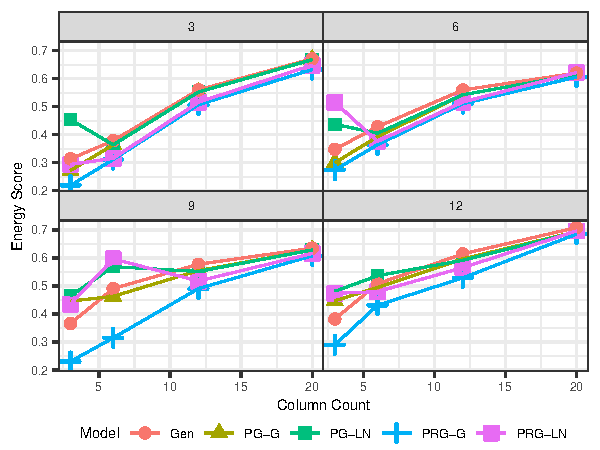
\includegraphics[width=0.8\textwidth]{./images/simulation_es}
% \end{figure}

\begin{figure}[ht]
  \begin{subfigure}[b]{0.45\textwidth}
    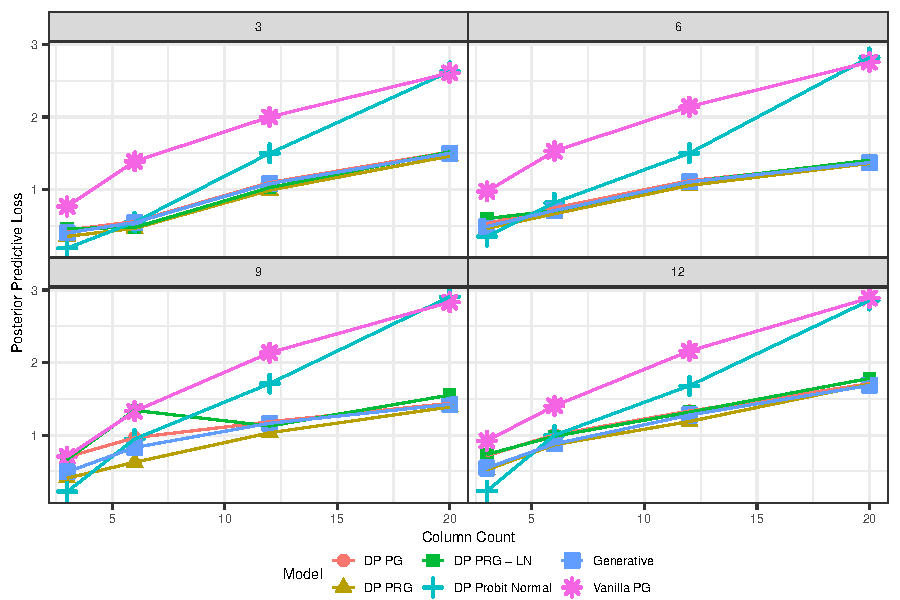
\includegraphics[width=\textwidth]{./images/simulation_ppl}
    \caption{Posterior Predictive Loss\label{fig:simppl}}
  \end{subfigure}
  %
  \begin{subfigure}[b]{0.45\textwidth}
    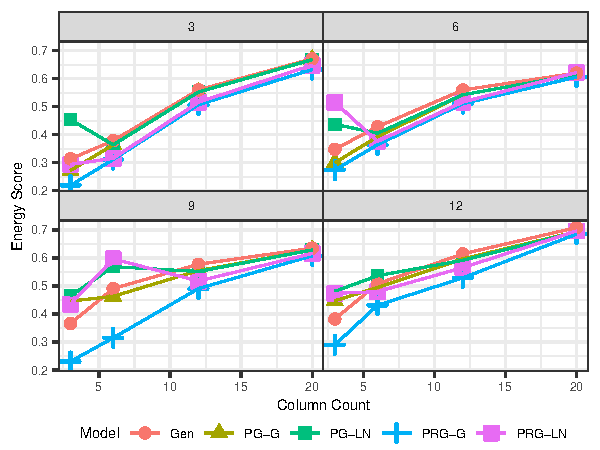
\includegraphics[width=\textwidth]{./images/simulation_es}
    \caption{Energy Score\label{fig:simes}}
  \end{subfigure}
  \caption{Simulation PPL (left) and ES (left) versus column count, by mixture component count.}
\end{figure}

In Figure~\ref{fig:simes}, we fit DP Mixtures of the various models presented and plot the resulting
  energy score against the number of columns, grouped by the number of mixture components used in
  dataset generation.  The \emph{Gen} model refers to a dataset generated
  in the same manner, from the same parameters as was used to create the original dataset.  Against
  this generative dataset, we compare DP Mixtures of projected gamma, projected restricted gamma, and
  projected restricted gamma with a multivariate log-normal prior.  We observe that the projected
  restricted Gamma model dominates in most situations, but the difference between projected restricted
  Gamma and the other gamma-based models tends to shrink as the number of columns increases.
  Alternatively, that difference appears to grow as the number of mixture components increases.

% \begin{figure}[ht]
%   \caption{Simulation posterior predictive loss versus column count, by mixture component count.\label{fig:simppl}}
%   \centering
%   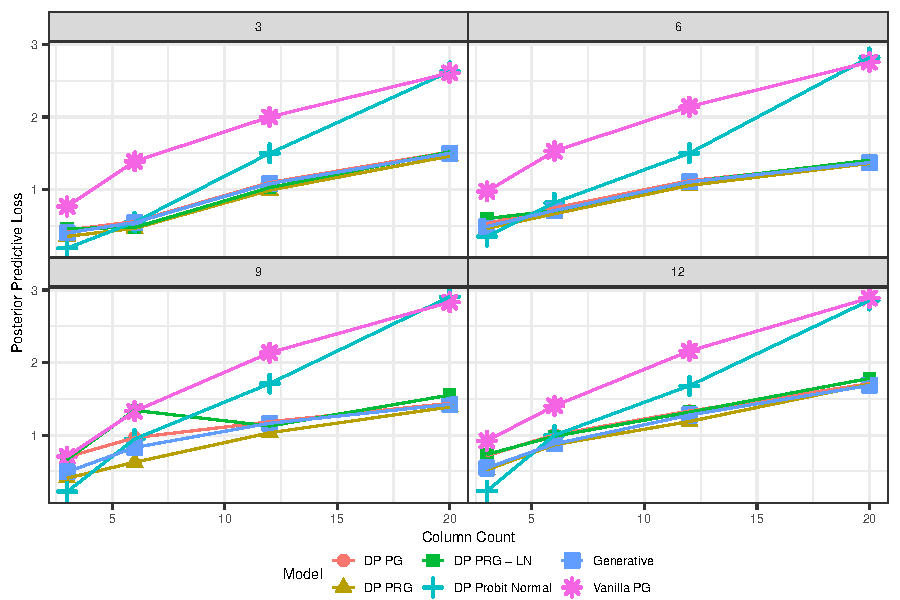
\includegraphics[width=0.8\textwidth]{./images/simulation_ppl}
% \end{figure}

The posterior predictive loss criterion in Figure~\ref{fig:simppl} tells a similar story: the base
  model is inadequate for describing a mixture; and the DP mixture of projected restricted gammas
  performs the best of the presented models in most cases.  Interestingly, under both metrics we see
  the probit-normal model has the best performance when the number of columns is low.  That is
  unexpected behavior, as its performance very quickly degrades as the number of columns increases.

We frequently see all of the gamma-based mixture models accomplish a lower energy score than the generative
  distribution.  As \cite{nunez2019} noted, the projected Gamma model is very flexible and can generate
  multimodal distributions from a single mixture component.  When we allow a mixture model, we allow
  the possibility to break those modes into two different mixture components.  This will tend to
  result in a better energy score, as posterior predictive replicates for a given observation in a local
  model will tend to be concentrate in that local mode rather than being spread between multiple
  modes.  As for the dominance of projected restricted Gamma, By specifying $\beta_{\ell} := 1$ for all
  $l$, if there were multi-modal mixture components, we are in effect breaking the mixture components
  into separate modes. As for whether this represents \emph{overfitting}, If we had reason to
  believe that the generative distribution for real data followed this form, then such a case could
  be made.  However, we are using projected Gamma as a parametric stand-in for an unknown distribution.
  In this sense, the argument for overfitting is less clear.

\subsection{Integrated Vapor Transport\label{subsec:ivt}}
The \emph{integrated vapor transport} (IVT) tracks the total water volume in a column of air over a given
  area \citep{ralph2017}.  IVT is the means by which we track the formation and path of atmospheric 
  rivers---elongated areas of high local concentration of water vapor in the atmosphere that moves with
  wind patterns.  Extreme behavior in IVT can lead to extreme precipitation events, causing flooding; 
  but in California, those same events are responsible for the bulk of precipitation that inland 
  California receives---water necessary for agriculture and household consumption.  Thus it becomes 
  necessary to manage precipitation to prevent inundation and support agriculture.  To this end, 
  understanding the dependence structure of extreme events in the IVT is useful---for instance, for 
  hydrological engineers in planning the capacity of groundwater systems to capture precipitation before 
  wasteful and destructive flooding occurs.  Our data tracks daily average values for the IVT, dividing 
  the coast of California into grid cells, with two spatial resolutions of 8 and 47 cells, respectively 
  \citep{guan2015}.

\begin{algorithm}[h]
  \KwResult{$\bm{ r},\bm{v} : r_i \sim \text{Pareto}(1)$, $\bm{ v}_i \in {\mathbb S}_{\infty}^{d-1}$}
  \For{$\ell = 1,\ldots,d$}{
    Set $b_{t,\ell} = \hat{F}_{\ell}^{-1}\left(1 - \frac{1}{t}\right)$.\\
    With $\bm{ x}_{\ell} > b_{t,\ell}$, fit $a_{\ell}$, $\chi_{\ell}$ via MLE according to generalized Pareto likelihood.\\
    }
  \For{$i = 1,\ldots,n$}{
    Define $z_{i,\ell} = \left(1 + \xi_{\ell}\frac{x_{i,\ell} - b_{t,\ell}}{a_{\ell}}\right)_{+}^{1/\xi_{\ell}}$\\
    Define $r_i = \pnorm{\bm{ z}_i}{\infty}$, $\bm{ v}_i = \frac{\bm{ z}_i}{\pnorm{\bm{ z}_i}{\infty}}$\\
    }
  Subset $\bm{ r},\bm{ v}$ such that $r_i \geq 1$\\
  \If{declustering}{
    \For{$i = 1,\ldots,n$}{
      If $r_i \geq 1$ and $r_{i-1} \geq 1$, drop the lesser (and associated $v_i$) from data set.\\
    }
  }
 \caption{Data preprocessing to isolate and transform data exhibiting extreme behavior.  $r_i$
   represents the radial component, and $\bm{v}_i$ the angular component.  The declustering
   portion is relevant if data is correlated in time.\label{algo:processing}}
\end{algorithm}

Fitting our models to this data requires some pre-processing. First, we subset the data to the rainy
  season, which appears from November to March.  The marginal distributions of the
  IVT data appear naturally log-normal, which falls into the domain of attraction of a Gumbel
  distribution.  Given that, we can apply a high threshold, and exceedances over that threshold can
  be modelled as Generalized Pareto.  Our modelling begins with that assessment.  As estimating
  the Pareto parameters is not yet our focus in this analysis, we choose to apply the threshold
  using the empirical CDF.  That is, for a given $t$, let $b_{t,\ell} = \hat{F}_{\ell}^{-1}(1 - t^{-1})$.  For
  this analysis, we set $t = 20$, indicating the marginal $95$ percentile.  The other parameters of the
  generalized Pareto---the scale parameter $\alpha_{\ell}$ and the extremal index $\chi_{\ell}$---are set via
  maximum likelihood. 

After the thresholding and maximum likelihood estimation of the parameters of the Pareto, we scale
  the data to the standard multivariate Pareto following Equation~\ref{eqn:standardization}.  
  Dividing each standardized observation by its $\mathcal{L}_{\infty}$ norm, we project the 
  standardized data onto $\mathcal{S}_{\infty}^{d-1}$. Data in sequence represents observations
  in time, which for this application are temporally correlated.  As such, we
  choose to \emph{decluster} the observations, such that, by observing a sequence of observations
  $\bm{ z}$ for which $\inorm{z_i} > 1$ for each observation in sequence, we keep only that observation
  with the greatest observed $\mathcal{L}_{\infty}$ norm.  The complete procedure is outlined in
  Algorithm~\ref{algo:processing}.  In the 8-cell data, after subsetting to the rainy season we 
  have $5587$ observations, which reduces to $511$ observations after processing and declustering.  
  In the 47 cell data, after subsetting we have $6342$ observations, which reduces to $532$ after 
  processing and declustering.  We fit PG--G, PRG--G, PG--LN, and PRG--LN models to both datasets.

\begin{table}[ht]
  \centering
  \caption{Model comparison metrics: Posterior Predictive Loss and Energy Score criteria from fitted
    models against the IVT data.  Lower is better.
  \label{tab:dev}}
  
\begin{tabular}{ccccc}
\toprule
\multicolumn{1}{c}{ } & \multicolumn{2}{c}{dim = 8} & \multicolumn{2}{c}{dim = 47} \\
\cmidrule(l{3pt}r{3pt}){2-3} \cmidrule(l{3pt}r{3pt}){4-5}
Model & PPL & ES & PPL & ES\\
\midrule
PRG & 0.195 & 0.170 & 1.623 & 0.675\\
PRG-LN & 0.232 & 0.192 & 1.400 & 0.582\\
PG & 0.787 & 0.418 & 5.040 & 1.374\\
\bottomrule
\end{tabular}
\end{table}

In Table~\ref{tab:dev} we see the same model preference towards the projected restricted 
  gamma models that we saw in Figures~\ref{fig:simes}.  The unrestricted gamma model is 
  penalized much more strongly on real data than we saw with our simulation.  We also see
  the restricted gamma model with the log-normal prior performing significantly better 
  than the restricted gamma model with the gamma prior on the higher dimensional data, a reversal
  of what we saw on the low dimensional data and indeed from what we saw in the simulation study.

\begin{figure}[ht!]
    \centering
    \caption{Pairwise extremal dependence coefficients for IVT data, from fitted PRG--G.  
    The left corresponds to the 8-cell data, the right the 47-cell data.\label{fig:chi_ij}}
    \begin{minipage}{.49\textwidth}
      \centering
      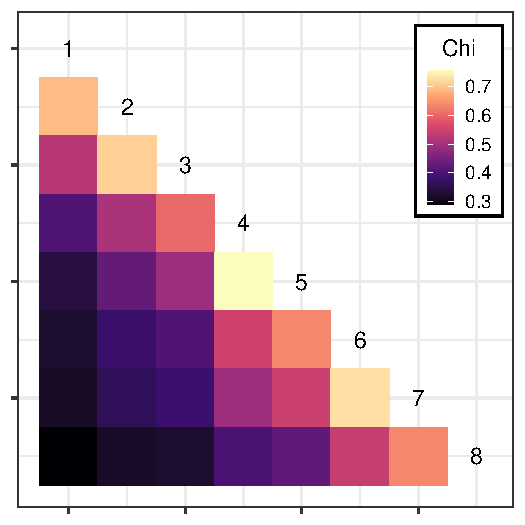
\includegraphics[width=0.99\linewidth]{./images/chi_ij_8}
    \end{minipage}
    \begin{minipage}{.49\textwidth}
      \centering
      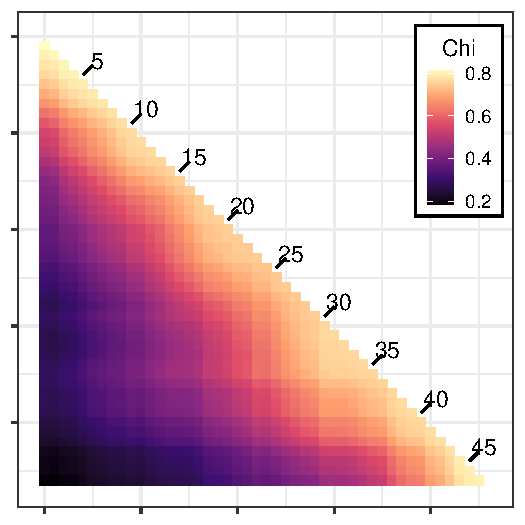
\includegraphics[width=0.99\linewidth]{./images/chi_ij_46}
    \end{minipage}
\end{figure}

Figure~\ref{fig:chi_ij} shows our implementation of Equation~\ref{eqn:chi_ij}, plotting the 
  pairwise extremal dependence coefficients for the IVT data computed from PRG--G models 
  fitted to the 8 (left) and 47 (right) cell data.  
  That we see a higher extremal dependence between neighboring columns is not unexpected, as
  neighboring columns correspond to neighboring cells.  We recognize that pairwise asymptotic
  dependence coefficients tell a limited story, as a particular dependence may structure may include
  more than two columns.   We can, however, glean some information from the patterns that emerge in
  two dimensions.  On the 8-cell data, we see a stronger association between cells 5-8, indicating a
  greater dependence among these cells.  On the 47 cell data, we see at least 3 groupings of columns,
  indicating greater asymptotic dependence among these groups.

 
% EOF
